\chapter{Choix technologiques}
	\section{Technologie back-end}
		\subsection{Symfony}
			\begin{center}
				
\includegraphics[scale=0.3]{chap_2/symfony.png}
				\captionof{figure}{Symfony}
				\label{Symfony}
			\end{center}
			Symfony est un framework de développement web open-source écrit en PHP. Il fournit un ensemble de composants modulaires et d'outils qui facilitent la création et la maintenance d'applications web complexes et évolutives. Symfony suit les principes de conception du modèle MVC (Modèle-Vue-Contrôleur), ce qui favorise la séparation des préoccupations et la structuration claire du code.\\
			Les caractéristiques principales de Symfony incluent :
			\begin{itemize}
				\item \textbf{Composants réutilisables} : Symfony est basé sur un ensemble de composants indépendants, tels que le gestionnaire de dépendances, le système de routage, le composant de formulaire, le composant de sécurité, etc. Ces composants peuvent être utilisés de manière modulaire dans différentes applications.
				\item \textbf{Productivité} : Symfony propose des outils et des générateurs de code qui accélèrent le développement. Il offre également une interface en ligne de commande (CLI) pour effectuer des tâches courantes telles que la génération de code, la gestion de bases de données et les tests.
				\item \textbf{Flexibilité} : Les développeurs peuvent personnaliser et configurer les composants selon les besoins spécifiques de leur projet. Symfony permet également l'intégration de bundles tiers pour ajouter des fonctionnalités supplémentaires.
				\item \textbf{Qualité du code} : Symfony encourage les bonnes pratiques de codage, le test unitaire et fournit des outils pour garantir la qualité du code. Cela facilite la maintenance à long terme des applications.
				\item \textbf{Sécurité} : Symfony offre des fonctionnalités de sécurité intégrées, telles que la gestion des autorisations, la protection contre les vulnérabilités courantes et la prévention des attaques.
				\item \textbf{Documentation} : Symfony dispose d'une documentation complète et détaillée, ainsi que d'une communauté active qui partage des ressources et des solutions aux problèmes courants.
				\item \textbf{Support à long terme} : Symfony suit des cycles de maintenance à long terme, ce qui garantit que les applications développées avec ce framework restent à jour et sécurisées.\\
			\end{itemize}
		
		Symfony est largement utilisé pour développer des applications web de toutes tailles, des sites web simples aux applications d'entreprise complexes. De nombreuses entreprises et projets renommés utilisent Symfony pour sa fiabilité, sa robustesse et sa capacité à accélérer le développement tout en maintenant des normes élevées de qualité et de sécurité.
		
		\subsection{PHPQA}
			\begin{center}
				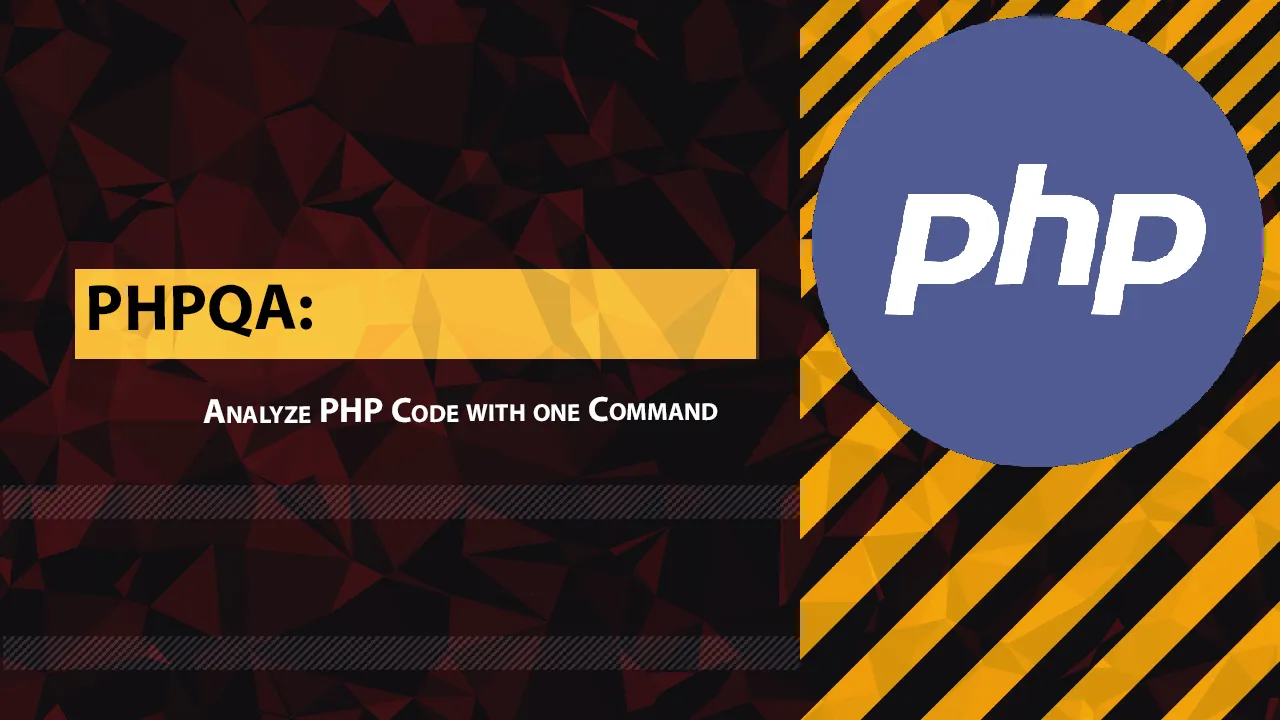
\includegraphics[scale=0.3]{chap_3/phpqa.png}
				\captionof{figure}{PHPQA}
				\label{PHPQA}
				\cite{phpqa_image}
			\end{center}
		
		PHPQA est un ensemble d'outils et de techniques destinés à l'analyse statique et dynamique du code PHP, ainsi qu'à l'amélioration de sa qualité et de sa performance. Il vise à aider les développeurs à identifier les problèmes potentiels dans le code, à maintenir de bonnes pratiques de développement et à optimiser les performances de leurs applications.
		
		Les principales catégories d'outils et de pratiques incluses dans PHPQA sont les suivantes :
		\begin{itemize}
			\item \textbf{Analyse statique du code} : Ces outils examinent le code source PHP sans l'exécuter et identifient des erreurs de syntaxe, des problèmes de sécurité, des antipatterns (mauvaises pratiques) et d'autres problèmes potentiels. Des exemples d'outils d'analyse statique populaires sont \textbf{PHPStan}, et \textbf{PHP CodeSniffe}r.
			\item \textbf{Mesure de la couverture de code} : Ces outils mesurent quelle partie du code est couverte par les tests automatisés, aidant ainsi à identifier les zones non testées et à garantir une meilleure couverture.
			\item \textbf{Profiler et analyseurs de performances} : Ces outils permettent de surveiller et d'analyser les performances de l'application en identifiant les goulots d'étranglement, les requêtes lentes et d'autres problèmes de performance. Des outils populaires incluent Xdebug et Blackfire.
			\item \textbf{Documentation du code} : La documentation claire et précise du code est importante pour la compréhension et la maintenance du projet. Des outils comme \textbf{PHPDocumentor} aident à générer une documentation automatique à partir des commentaires du code source.
			\item \textbf{Amélioration du style de code} : Les outils comme \textbf{PHP CS} Fixer aident à maintenir un style de code cohérent en automatisant la correction des espaces, des indentations et d'autres conventions de codage.
		\end{itemize}
		
		En utilisant PHPQA, les développeurs peuvent identifier rapidement les problèmes potentiels dans leur code, améliorer sa qualité, accélérer le processus de développement et optimiser les performances de leurs applications PHP. Cela contribue à créer des applications plus robustes, fiables et performantes.
		
		
		\subsection{Codeception}
			\begin{center}
				
\includegraphics[scale=1]{chap_3/codeception.png}
				\captionof{figure}{Codeception}
				\label{Codeception}
				\cite{codeception_image}
			\end{center}
		Basé sur PHPUnit, Codeception est un framework de test automatisé pour les applications web. Il est principalement utilisé pour effectuer des tests unitaires, fonctionnels et d'acceptation dans le contexte du développement web. Codeception simplifie la création et l'exécution de tests automatisés en fournissant des fonctionnalités spécifiques pour l'émulation d'actions utilisateur, la validation du comportement de l'application.\\
		Aussi, il rassemble et partage les meilleures pratiques et solutions pour tester les applications web PHP. Grâce à un ensemble flexible de modules inclus, les tests sont faciles à écrire, à utiliser et à maintenir \cite{codeception}.\\
		En plus d'offrir les fonctionnalités de PHPUnit, codeception offre de modules intéressants permettant de faire facilement des tests d'acceptance et fonctionnels.
		
		\subsubsection{Docker}
			\begin{center}
				
\includegraphics[scale=1]{chap_3/docker.jpg}
				\captionof{figure}{Docker}
				\label{Docker}
				\cite{docker_image}
			\end{center}
		Docker est une plate-forme open-source qui permet de développer, déployer et exécuter des applications dans des conteneurs légers et portables. Les conteneurs sont des environnements logiciels isolés qui incluent tout ce dont une application a besoin pour s'exécuter, y compris le code, les bibliothèques, les dépendances et les configurations.\\
		Docker permet aux développeurs d'être sur la même longueur d'onde en terme de version de logiciels utilisées lors de la phase de développement. Ce qui peut être très utile pour éviter de potentiels problèmes lors du déploiements d'une application.
		
		
		\subsection{MariaDB}
			\begin{center}
				
\includegraphics[scale=0.5]{chap_3/mariadb.png}
				\captionof{figure}{Docker}
				\label{MariaDB}
				\cite{mariaDB_image}
			\end{center}
		MariaDB est un système de gestion de base de données open-source et relationnel (SGBDR) qui est conçu pour être une alternative compatible avec MySQL. Il a été créé par certains des développeurs originaux de MySQL en réponse à des préoccupations concernant la direction et la gouvernance de MySQL après son acquisition par Oracle Corporation.\\
		MariaDB partage une grande partie de la syntaxe et des fonctionnalités avec MySQL, ce qui signifie que les applications écrites pour MySQL peuvent généralement être utilisées avec MariaDB sans modifications majeures. Cependant, MariaDB propose également des améliorations et des fonctionnalités spécifiques qui en font une option attrayante pour de nombreux utilisateurs.\\
		Les avantages principaux qu'on peut tirer de MariaDB sont:
		\begin{itemize}
			\item \textbf{Performance} : MariaDB inclut des optimisations et des améliorations de performances par rapport à MySQL, notamment dans les domaines de la vitesse d'exécution des requêtes et de la gestion de la mémoire.\cite{chatgpt}
			\item \textbf{Stockage} : MariaDB prend en charge divers moteurs de stockage, y compris InnoDB (le moteur de stockage par défaut), Aria, MyISAM et d'autres.\cite{chatgpt}
			\item \textbf{Haute disponibilité} : MariaDB propose des fonctionnalités de réplication et de clustering pour garantir une haute disponibilité des données et une tolérance aux pannes, etc.\cite{chatgpt}
		\end{itemize}
	
	\section{Technologie back-end}
		\subsection{AdminLTE}
			\begin{center}
				
\includegraphics[scale=0.7]{chap_3/adminlte.png}
				\captionof{figure}{AdminLTE}
				\label{AdminLTE}
				\cite{adminlte_image}
			\end{center}
		AdminLTE est un template open-source de conception d'interface utilisateur (UI) et d'administration pour les applications web. Il fournit une collection de composants, de styles CSS et de scripts JavaScript préconstruits pour créer rapidement des interfaces d'administration élégantes et conviviales.\\
		L'avantage avec Admin Lte, c'est qu'il permet aux développeurs avoir d'un gain de temps énorme et de se concentrer sur la logique métier de l'application, du fait des composants réutilisables mis à leur disposition.
		
		\subsection{ChartJS}
			\begin{center}
				
\includegraphics[scale=0.5]{chap_3/chartjs.png}
				\captionof{figure}{ChartJS}
				\label{ChartJS}
				\cite{chartjs_image}
			\end{center}
			ChartJS est une bibliothèque JavaScript open source gratuite pour la visualisation de données. Créée par le développeur web Nick Downie en 2013, la bibliothèque est maintenant maintenue par la communauté et est la deuxième bibliothèque de graphiques JS la plus populaire sur GitHub par le nombre d'étoiles après D3.js. Chart.js est rendu dans un canvas HTML5. Elle est disponible sous la licence MIT.\cite{chartjs}\\
			Pour réaliser les diagrammes d'évolutions et les courbes de tendance, ChartJS a été un élement essentiel, voir indispensable.
			
		\subsection{ReactJS}
			\begin{center}
				
\includegraphics[scale=0.4]{chap_3/react.png}
				\captionof{figure}{React}
				\label{ReactJS}
				\cite{react_js}
			\end{center}
			React JS est une biblithèque javascript développée par Facebeook depuis 2013 \cite{react_wiki}. Il offre la de possibilité de créer des composants réactive grâce aux hooks. React a pour avantage d'être utilisé en fonction de l'état d'un projet (from scratch ou en plein milieu). Pour un projet demarré à partir de zéro, il est possible de créer une application full-react, dont la mise en place est juste éffectuée par une commande (\textbf{create-react-app}).\\
			Dans le cas de notre application il a été utilisé (grâce à Symfony UX) pour rendre le tableau des bluids plus réactif à chaque clique d'un utilisateur.	